\documentclass[11pt, a4paper]{article}

\usepackage[utf8]{inputenc}
\usepackage{authblk}
\usepackage{titlesec}

% Maths tools
\usepackage[tbtags]{amsmath}
\usepackage{amssymb}

% Margin
\usepackage[margin=2.9cm]{geometry}

% Line numbers
\usepackage{lineno}

%Scientific notation
\usepackage{siunitx}

% Landscape page
\usepackage{pdflscape}
\usepackage{afterpage}

% Spacing
\usepackage{setspace}
\doublespacing

% Enumeration
\usepackage{enumerate}

% indentation
\setlength\parindent{10pt}
\setlength{\parskip}{5pt}

% Figures
\usepackage{graphicx}
\usepackage{caption}
\usepackage{subcaption}
\usepackage{epstopdf}
\renewcommand{\thefigure}{\textbf{\arabic{figure}}}
\renewcommand{\figurename}{\textbf{Supplementary Figure}}

%table
\usepackage{multirow}
\usepackage{hhline}
\usepackage[table]{xcolor}
\renewcommand{\thetable}{\textbf{\arabic{table}}}
\renewcommand{\tablename}{\textbf{Supplementary Table}}

%footnotes
\usepackage{footmisc}
\renewcommand{\thefootnote}{\fnsymbol{footnote}}

% References
\usepackage[sort&compress, numbers,super]{natbib}
\bibliographystyle{unsrtnat}
\PassOptionsToPackage{hyphens}{url}\usepackage[colorlinks=true,linkcolor=magenta, citecolor=magenta]{hyperref}
\renewcommand\refname{Supplementary References}

%subsubsection format
\titleformat*{\subsubsection}{\large\it}

%highlighting text
\usepackage{color, xcolor,soul}
\definecolor{blau}{RGB}{236,226,240}
\soulregister\cite7
\soulregister\citet7
\soulregister\citealt7
\soulregister\citenum7
\soulregister\citep7
\soulregister\ref7
\DeclareRobustCommand{\hlc}[1]{{\sethlcolor{blau}\hl{#1}}}

\usepackage{makecell}

\usepackage{titlesec}% http://ctan.org/pkg/titlesec
\titleformat{\section}%
  [hang]% <shape>
  {\normalfont\bfseries\Large}% <format>
  {}% <label>
  {0pt}% <sep>
  {}% <before code>
  
\renewcommand{\thesection}{}% Remove section references...
\renewcommand{\thesubsection}{}%... from subsections
  \renewcommand{\thesubsubsection}{Supplementary Method \arabic{subsubsection}:}%... from subsections

\renewcommand{\arraystretch}{1.3}
  
%Title paper
\title{\vspace{-1cm} \normalsize Supplementary Information\\\vspace{0.2cm}
\LARGE Using Bayesian non-linear models to uncover broad macroecological patterns}

\author{\textit{Bramon Mora et.\,al.}}

\date{}

\begin{document}
\maketitle
\thispagestyle{empty}

\clearpage

% Full description of Binomial model with multiple environmental covariates
% Full description of Categorical model with multiple environmental covariates
% Full description of Categorical model with heavy-tails---generalized error distribution
% Full description of Categorical model with heavy-tails---Student's t-distribution
% Full description of Categorical model with skewed---skewed normal distribution
% Using a MMSBM to calculate species similarity
% Edge problem in stan and need to define minimum probability.

\section*{Supplementary Methods}
\subsubsection*{Full description of the baseline model}
While the baseline model described in the main text included only one predictor, the same model can be extended to include multiple environmental variables. For example, imagine that we had $k$ predictors describing the environmental conditions of any given site $j$. The baseline model in Eq.~(1) of the main text could then be rewritten as:
\begin{equation}
\begin{split}
y_{ij} & \sim \text{Binomial}\left(1, p_{ij}\right) \\
\text{log}\left(p_{ij}\right) & = -\alpha_{i} - \sum_k \gamma_{ik} \left(x_{jk}-\beta_{ik}\right)^2,
\end{split}
\label{eq:baseline-binary}
\end{equation}
where $y_ij$ describes the presence and absence of species, and the prior distributions for the different parameters are analogous to the ones described in the main text.

Similarly, if the response variable $y_ij$ represented ordinal data (e.g.~Braun-Blanquet abundance-dominance classes), characterized by $K$ different classes. Then, one can adapt Supplementary Eq.~(\ref{eq:baseline-binary}) as:
\begin{equation}
\begin{split}
y_{ij} & \sim \text{Categorical}\left(\mathbf{q}\right) \\
q_{1} & = 1- p_{ij}\phi_1 \\
q_{k} & =  p_{ij}\phi_{k-1} -  p_{ij}\phi_{k} \\
q_{K} & =  p_{ij}\phi_{K-1} \\
\text{log}\left(p_{ij}\right) & = -\alpha_{i} - \sum_k \gamma_{ik} \left(x_{jk}-\beta_{ik}\right)^2 \\
\phi_1 & = \hat{\phi_1} \\
\phi_k & = \hat{\phi_k} \,\, \hat{\phi_{k-1}} \\
\hat{\phi} & = \text{Beta}(1,1),
\end{split}
\label{eq:baseline-categorical}
\end{equation}
where the prior distributions for the rest of parameters are analogous to the ones described in the main text.

\subsubsection*{Distance matrices from incomplete categorical and ordinal data}
The prior information that we have regarding species' distributions is represented by the set of ordinal and categorical traits found in the attributes database. More specifically, both the ecological indicator values and range of variation are ordinal traits, containing potential missing entries (Supplementary Table \ref{stab:EI}). These data could be directly used as covariates in any given distribution model; however, we want this information to be accounted for as a prior for the relevant parameters of our Bayesian model. One way to do so is by compiling the traits in the attributes database into variance-covariance matrices characterizing the \textit{a priori} similarity between species. To accomplish this, we need to turn the set of ecological indicator values and range of variation into the distance matrices $D$ presented in the text.
%, whereas plants' physiological data are characterized by categorical data containing multiple missing entries.

More generally, we want to understand the way $N$ species are characterized by $M$ categorical traits. One way to frame this problem is by using a network representation. Following the ideas presented by \citet{godoy-loriteAccurateScalableSocial2016}, we assume that species can be connected to each of these traits by an interaction $\left(i, j\right)$ that can be of any type $r\in R$. Notice that this provides us with multiple ways to account for the information---and lack thereof---contained in the different ordinal traits $M$. That is, the $R$ types of interactions can represent the lack of information for a particular link $\left(i, j\right)$, the absence or presence of such interaction, and any type of association between $i$ and $j$. Then, given a set of interactions $R^{*}$ between $N$ and $M$, we can use a Mixed Membership Stochastic Block Model (MMSBM) to understand the differences between species. In particular, these models consider that the $N$ plants and $M$ traits can be classified into $K$ and $L$ groups types, respectively. Then, they estimate `group-membership vectors', describing the extend to which the different plants and traits belong to the different group types.

Here, we use the MMSBM presented by \citet{godoy-loriteAccurateScalableSocial2016}, and classify plants into 5 types of species, and traits into 5 trait groups. Then, we estimate the group-membership vectors $\vec{\theta}_{\text{plants}}$, and calculate the pairwise distances $D_{ij}$ between plants as the euclidean distance between their membership vectors.  We run these models independently for species' ecological indicator values and their range of variation (Supplementary Table \ref{stab:EI}) to generate the two distance matrices for parameters $\beta_i$ and $\gamma_i$. Notice that the MMSBM uses an expectation-maximization algorithm to estimate the different membership vectors. Therefore, in order to have good estimates of the different pairwise distances $D_{ij}$ for $\beta_i$ and $\gamma_i$, one needs to run the MMSBM several times (1000 times) and average the resulting pairwise distances \citep{godoy-loriteAccurateScalableSocial2016, tarres-deulofeuTensorialBipartiteBlock2019}. 

This type of classification of ordinal variables that describe different species can also be done with other algorithms, including categorical PCA and matrix factorization methods. However, the MMSBM provides a convenient tool to classify very different types of traits, including categorical variables or diverse data containing multiple missing entries. Moreover, MMSBM have been shown to better capture the patterns of this sort of data \citet{godoy-loriteAccurateScalableSocial2016}.

%Given a set of interactions $R^{*}$ between $N$ and $M$, we use a Mixed Membership Stochastic Block Model (MMSBM) to characterize these. In particular, we consider that plants and traits can be classified into $K$ and $L$ groups, respectively. For every species $i$, we assume that there is a probability $\theta_{i\alpha}$ for it to belong to any of the $K$ species groups. Likewise, we also assume that any trait $j$ has a probability $\phi_{j\beta}$ of belonging to any of the $L$ trait groups. Finally, we define $p_{\alpha\beta}\left(r\right)$ as the probability of a species from group $\alpha$ interacting with a trait from group $\beta$ by an association type $r$. Putting these together, the probability of an interaction $\left(i, j\right)$ of type $r$ can be calculated as:
%\begin{equation}
%Pr[r_{ij}=r] = \sum_{\alpha \beta} \theta_{i\alpha} \phi_{j\beta} p_{\alpha\beta}\left(r\right)
%\end{equation}
%Following this definition, we want to find the group memberships that maximize the likelihood $P\left(R^{*}|\theta, \phi, p\right)$. Doing so is difficult optimization problem; however, it has been shown that one can estimate the different $\theta_{i\alpha}$, $\phi_{j\beta}$, and $p_{\alpha\beta}\left(r\right)$ parameters by maximizing the likelihood using an expectation-maximization algorithm \citep{godoy-loriteAccurateScalableSocial2016, tarres-deulofeuTensorialBipartiteBlock2019}. In simple terms, one can iteratively find multiple local minima for the likelihood, and average over the estimated the parameter values \citep{godoy-loriteAccurateScalableSocial2016}\footnote[2]{
%While this averaging is trivial for the estimated probabilities $Pr[r_{ij}=r]$, it is non-trivial if one wants to find averages for the group memberships. The reason for this is related to the stochastic nature of the expectation-maximization algorithm. This algorithm initially assigns random group memberships to both species and traits. While this random labelling is irrelevant when studying the probabilities $Pr[r_{ij}=r]$, it is instead crucial for averaging $\theta_{i\alpha}$, $\phi_{j\beta}$, and $p_{\alpha\beta}\left(r\right)$. Therefore, before averaging the group membership estimates, one needs to find the bijective relationship for the labellings of different iterations of the optimization algorithm. In a nutshell, for every iteration, I do this by using a simulated annealing algorithm on the estimated $p_{\alpha\beta}\left(r\right)$, matching the corresponding labelling to a reference iteration.}. 

%The average estimates for the group memberships provide us with a different scale to classify species based on the traits these have. In short, for any species $i$, we can estimate a $K$-dimensional vector $\vec{\theta}_{i}$ that describes the extend to which $i$ belong to each group membership---i.e. the extend to which a species is of one type or another. This classification is useful because it can be used to compare species, defining a way to measure the distance between species based on an arbitrary---and potentially incomplete---set of categorical or ordinal traits $M$. The simplest case is to define the distance as $D_{ij} = |\vec{\theta}_{i}-\vec{\theta}_{j}|$. Alternatively, one could also define $K$ distance matrices based on the different group memberships $D^{\alpha}_{ij} = |\theta_{i\alpha}-\theta_{j\alpha}|$.

%\subsubsection*{Sampling the posterior: simulated data and additional information}
%A good way to understand the model behaviour and the choice of prior distributions is by using simulated data. Here, we only present the simulations for the baseline model---the simplest model---but similar simulations were done for the others (see Code Availability section of the main text). 
%
%To simulate the data, we first generated two distance matrices relating the different parameters

\subsubsection*{Alternative variance-covariance structures}
The model structure defined above allows us to test how different sources of information characterize each of the different parameters. For example, imagine that we have multiple matrices $D^k$ characterizing species' differences along different axis of variation---e.g.~two matrices characterizing physiological and environmental traits. One can modify Eq.~(3) of the main text for a particular parameter---e.g.~$\beta_{i}$---such that
\begin{equation} 
\Sigma_{ij} = \eta\,\text{exp}\left(-\sum_k\rho_{k} {D^{k}_{ij}}^2\right) + \delta_{ij} \sigma ,
\label{eq:covariance-complex}
\end{equation}
where now $\rho_{k}$ are separate relevance hyperparameters for each distance matrix in the total variance of $\beta_i$.

\section*{Supplementary Notes}
\subsubsection*{Supplementary Note 1: studying the hyperparameters of the Gaussian processes}
As described in the main text, we use Gaussian processes to account for the prior information regarding a given parameter (e.g.~$\beta_i$), characterized by a distance matrix $D$ (see `Distance matrices from incomplete categorical and ordinal data' section of the Supplementary Methods). The advantage of using a Gaussian processes is that one can assess the value of the prior information by studying the posterior distributions of the corresponding hyperparameters. As described in Eq.~(3) of the main text, the hyperparameter $\rho$ of a Gaussian process determines the rate of decline of the covariance between any two species, $\eta$ defines its maximum value, and $\sigma$ describes the additional covariance between the different observations for any given species. Therefore, the higher the $\eta$ values relative to $\sigma$ (for $\rho>0$), the more the prior knowledge informs the parameter values of the different species. 

In all models, we use species' environmental indicator values and range of variation to inform the parameters $\beta_i$ and $\gamma_i$, respectively. Supplementary Fig.~\ref{sfig:hyperparameters1} displays the posterior distributions for $\eta$, $\rho$ and $\sigma$ for each parameter, calculated using the model with fat-tailed and skewed shape. Notice that the environmental indicator values are much more informative to the $\beta_{i}$ parameters than the species' range of variation is to the $\gamma_{i}$ parameters. This is potentially due to the fact the environmental indicator values have higher resolution that the information regarding species' range of variation in the attributes database. 

The information obtained in Supplementary Fig.~\ref{sfig:hyperparameters1} is not particularly surprising, as we already expected our prior knowledge to be somewhat informative to both $\gamma_{i}$ and $\beta_{i}$ parameters. However, this figure highlights the potential for understanding the extend to which different sources of data inform the different aspects of the shape of distributions. For example, imagine that we had trait information on the different species. We could use a Gaussian process to characterize the $\lambda_i$ parameters, using this information as our prior knowledge. The hyperparameters of this Gaussian processes could then reveal the extend to which some ecological traits explain the skewness of species distributions.

\subsubsection*{Supplementary Note 3: validation of $\lambda$ estimates}

One could hypothesise that the level skewness of distributions depends on the fact that some species can be found near the edge of the sampling area. However, the advantage of using a Bayensian approach to study such distributions is that we obtain full descriptions of the parameter posterior distributions, and we don't make any assumptions regarding the nature of the distributions outside of the sampling area. Therefore, a species that is near the edge of the sampling area should only result in larger confidence intervals for some of the parameter estimates, as it only implies less certainty regarding the true shape of such species' distribution. To showcase this, we used two strategies: studying subsets of the original data and using simulated data.

To study subsets of the data, we considered different windows of elevation containing 25\% of the data. To do so, given the distribution of site elevation, we divided our dataset into 5\% subsets $s_{i}$. This means that, for example, $s_1$ and $s_{20}$ contain the 5\% of sites at the lowest and highest elevations, respectively. Using these subsets of data, we grouped them to consider 16 elevation windows containing 25\% of the data, so that the first window of elevation contains all subsets of data between $s_1$ and $s_5$, the second window contains the subsets between $s_2$ and $s_6$; and so on. Then, we used the model characterized by fat-tails and a skewed response curve, and analysed the distribution of species in each elevation window, independently (considering those species with at least 20 occurrences). Finally, focussing on the parameter characterizing the skewness of distributions $\lambda_i$, we compared the posterior distributions obtained for each window of elevation with those obtained using the full dataset. In particular, we focused on whether or not the mean parameter values obtained using the full dataset fell within the confidence intervals of the posterior distributions obtained using the different windows of elevation. As expected, we found this to be true in $>99\%$ of the cases, which highlights the fact that sampling edges might add uncertainty to our estimates but does not make additional assumptions regarding the nature of the data.

Another way to validate the predictions of the model is by using simulated data. To do so, one can generate species' distribution data using a skewed generalized error distribution (see Code availability section), and compare the true values to the estimated posterior distributions. Supplementary Fig.~\ref{sfig:simulated-lambdas} displays the results for 50 simulated species distributions for $\beta_i$ and $\lambda_i$. Notice that the model does a good job characterizing the true $\lambda_i$ values in most cases (with the exception of some simulated species with low number of occurrences $<20$). This is important because it shows that with limited data, the model does a good job predicting the true values of $\lambda_i$ despite the variation in $\alpha_i$, $\gamma_i$, $\beta_i$, $\nu_i$. Perhaps most importantly, we generated the simulated data assuming that $\text{logit}\left(\frac{\lambda_i+1}{2}\right)\sim\text{Normal}(1, 0.5)$ (see Code Availability section). That is, the simulated lambdas are generally positive (i.e.~skewed in the same direction).  Notice that the posterior distributions are not affected by the $\beta_i$ parameters (i.e.~the center of the distributions), and are consistently predicted to be above zero.


\section*{Supplementary Figures}

\begin{figure}[ht]
  \centering
    \vspace{0.5cm}
    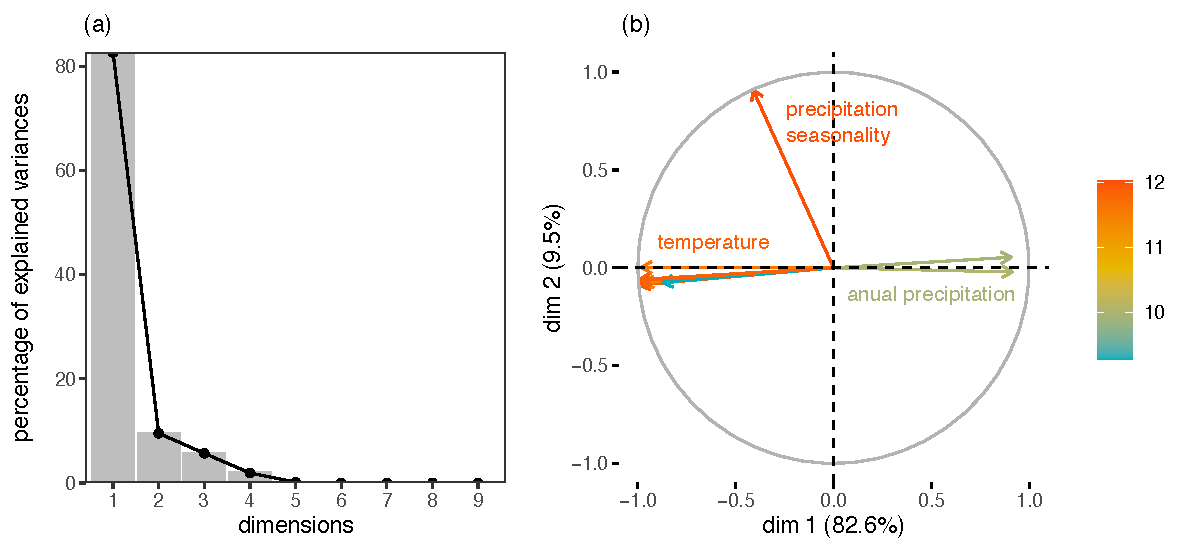
\includegraphics[width=1\textwidth]{figures/variances}
    	  \vspace{0.3cm}
	   \caption{Principal components analysis of the different environmental variables used. Panel (a) displays the percentage of variation explained by each principal component. Panel (b) provides a visualization of the contribution of each variable to the first two axes of variation. These graphs were generated using R functions from the package `factoextra' \citep{kassambaraFactoextraExtractVisualize2017}}.
      \label{sfig:pca}
\end{figure}

\clearpage

%\begin{figure}[ht]
%  \centering
%    \vspace{0.5cm}
%    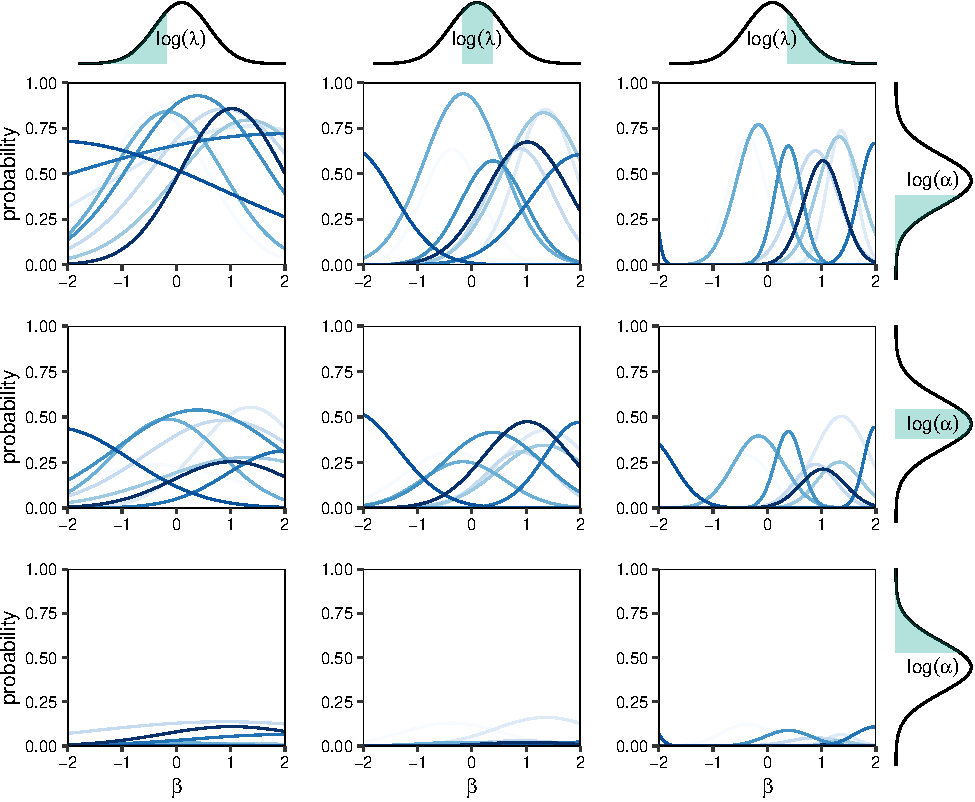
\includegraphics[width=1\textwidth]{figures/prior}
%    	  \vspace{0.3cm}
%	   \caption{Study of the priors for the baseline model presented in the main text.}
%     \label{sfig:sensitivity}
%\end{figure}
%\clearpage

\begin{figure}[ht]
  \centering
    \vspace{0.5cm}
    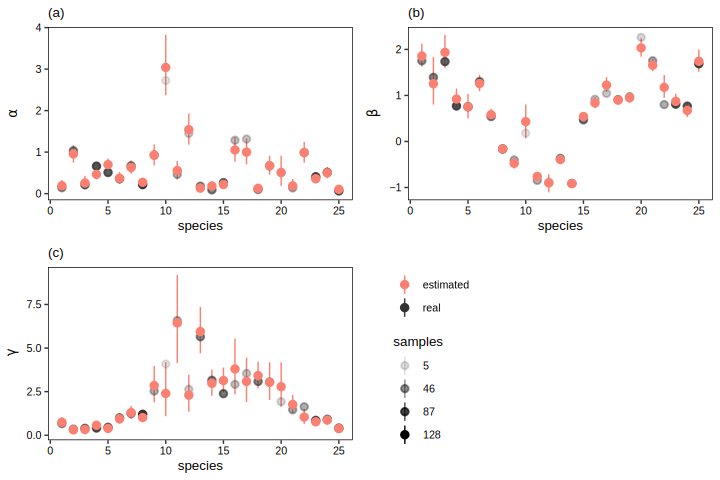
\includegraphics[width=1\textwidth]{figures/simulations-comparison}
    	  \vspace{0.3cm}
	   \caption{Testing the baseline model's performance with simulated data. We generated 25 bell-shaped distributions along an environmental axis, randomly sampling the different parameter values $\alpha_i$, $\beta_i$ and $\gamma_i$. More specifically, the $\text{log}\left(\alpha_i\right)$ parameters were sampled from a normal distribution with mean $-0.5$ and variance $1$; the $\beta_i$ and $log(\gamma_i)$ parameters were instead sampled from two multivariate normal distributions so that the covariance between species 1 and 2 is larger than the covariance between species 1 and 3 (see Code Availability section for further information). Then we used these distributions to simulate presence/absence data along the environmental axis using a binomial distribution, and used the baseline model to estimate the posterior distributions for the different parameters. The different panels showcase the comparison between real parameter values (black) and the posterior distributions (red) for (a) $\alpha_i$, (b) $\beta_i$, and (c) $\gamma_i$. The transparency for the points describing the real parameter values provides an indication of the sample size of each simulated species (number of occurrences). The red dots and red bars characterize the mean and the $89\%$ confidence intervals for the different posterior distributions, respectively.}
      \label{sfig:simulations}
\end{figure}

\clearpage

\begin{figure}[ht]
  \centering
    \vspace{0.5cm}
    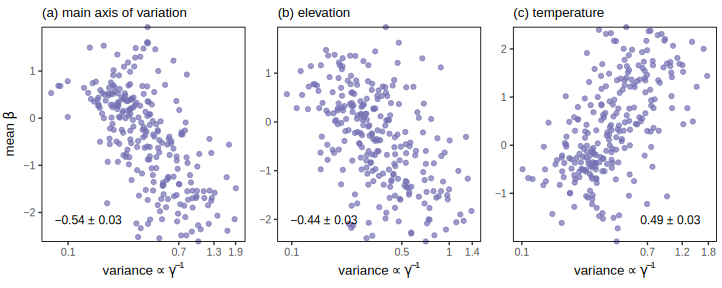
\includegraphics[width=1\textwidth]{figures/pca-elevation-temperature}
    	  \vspace{0.3cm}
	   \caption{Relationship between the posterior distributions for parameters $\beta_i$ and $\gamma_i$ across species considering different environmental variables. Panel (a) describes the relationship between the mean ($\beta_i$) and variance ($\propto\gamma_i^{-1}$) of distributions along the main axis of variation in Supplementary Fig.~\ref{sfig:pca}. Panel (b) and (c) describes the same relationship along elevation and average temperature. Each point represents the average value of the corresponding posterior distributions for any given species. The value in the bottom-left corner of the plot displays the Pearson's correlation coefficient between the parameters calculated across all samples.}
      \label{sfig:temperature-elevation}
\end{figure}

\clearpage

\begin{figure}[ht]
  \centering
    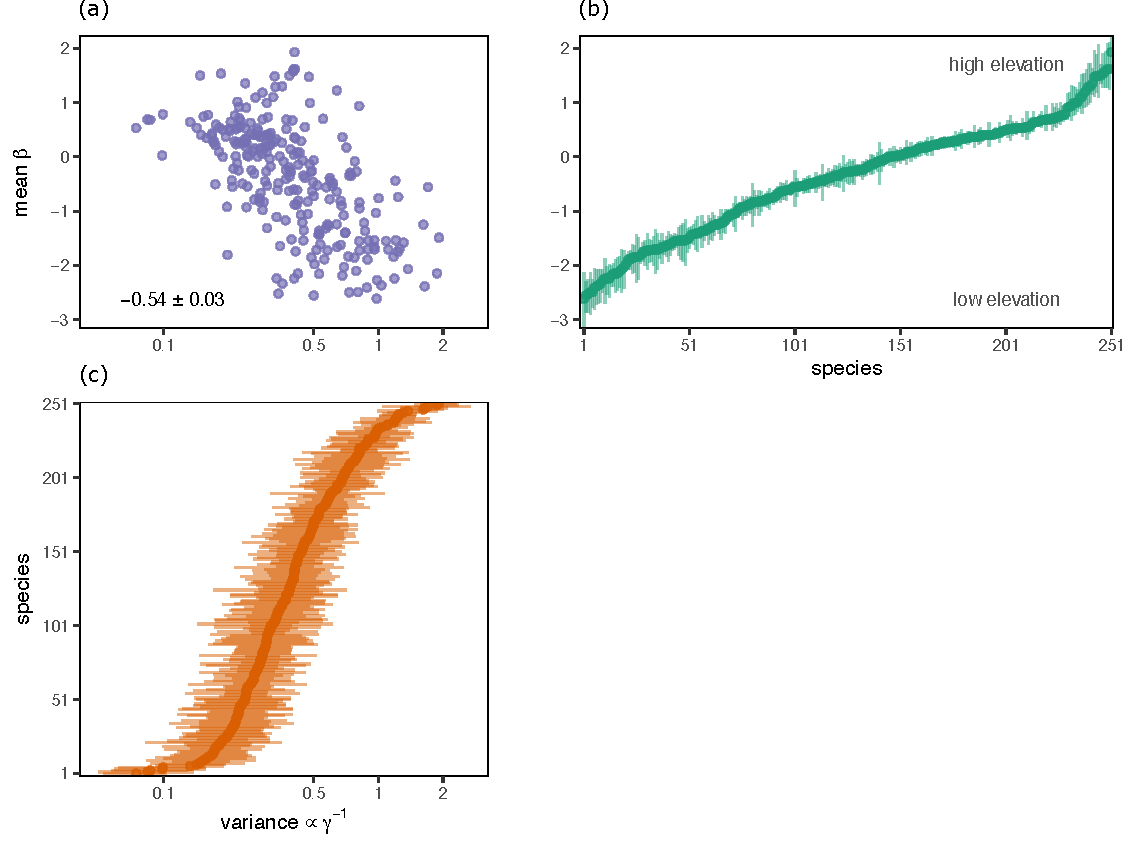
\includegraphics[width=0.95\textwidth]{figures/categorical-figure1}
    	  \vspace{0.1cm}
	   \caption{Relationship between the posterior distributions for parameters $\beta_i$ and $\gamma_i$ across species. These results are analogous results to those displayed in Fig.~2 of the main text, but they were obtained using ordinal measures of abundance instead of presence/absence data. Panel (a) describes the relationship between the mean ($\beta_i$) and variance ($\propto\gamma_i^{-1}$) of distributions. Each point represents the average value of the corresponding posterior distributions for any given species. The value in the bottom-left corner of the plot displays the Pearson's correlation coefficient between the parameters calculated across all samples. Panel (b) displays the estimates for the center of species' distributions along the environmental gradient. Panel (c) displays the estimates for the variance of species' distributions along the environmental gradient. In (b) and (c), the points represent the mean of the posterior distributions, the corresponding lines characterize the 89\% confidence intervals, and species are sorted according to the mean of the posterior distributions along the x and y axes, respectively.}
	   %7.5-4
      \label{sfig:categorical-baseline}
\end{figure}

\clearpage

\begin{figure}[ht]
  \centering
    \vspace{0.5cm}
    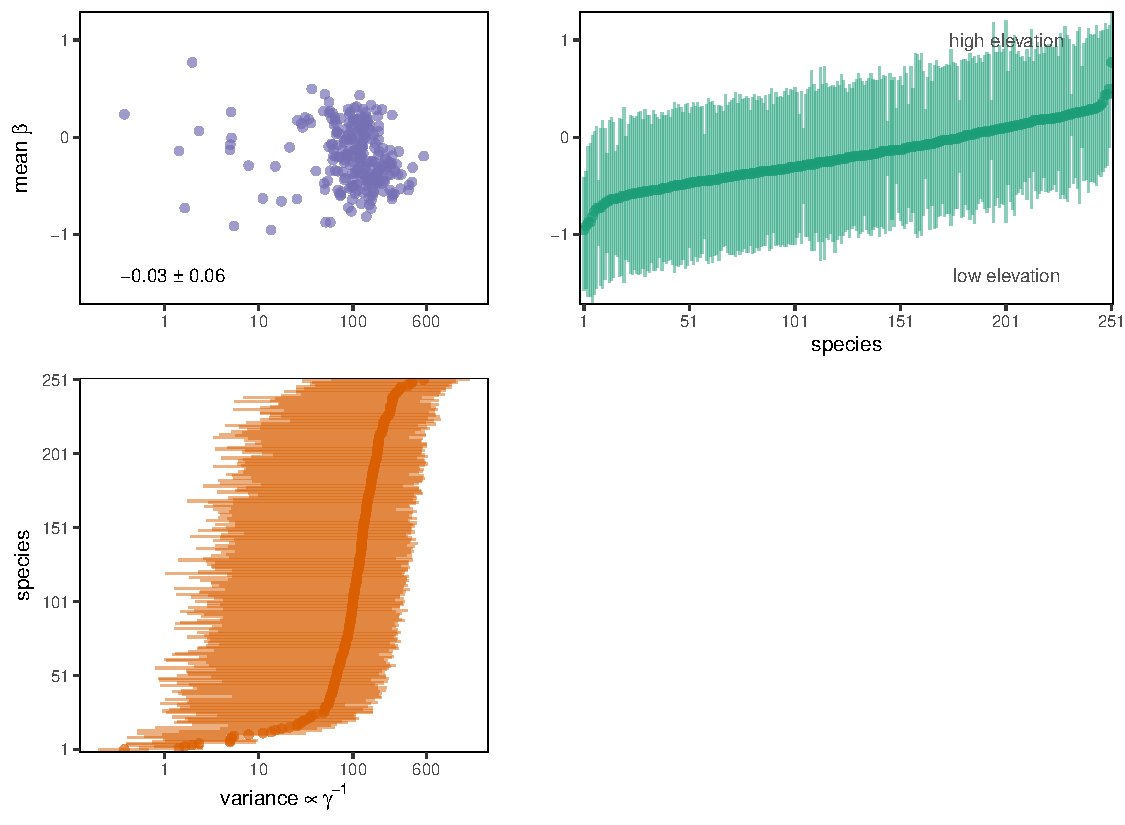
\includegraphics[width=1\textwidth]{figures/figure1-secondaxis}
    	  \vspace{0.3cm}
	   \caption{Relationship between the posterior distributions for parameters $\beta_i$ and $\gamma_i$ across species along the second axis of variation in Supplementary Fig.~\ref{sfig:pca}. Panel (a) describes the relationship between the mean ($\beta_i$) and variance ($\propto\gamma_i^{-1}$) of distributions. Each point represents the average value of the corresponding posterior distributions for any given species. The value in the bottom-left corner of the plot displays the Pearson's correlation coefficient between the parameters calculated across all samples. Panel (b) displays the estimates for the center of species' distributions along the environmental gradient. Panel (c) displays the estimates for the variance of species' distributions along the environmental gradient. In (b) and (c), the points represent the mean of the posterior distributions, the corresponding lines characterize the 89\% confidence intervals, and species are sorted according to the mean of the posterior distributions along the x and y axes, respectively.}
      \label{sfig:secondaxis}
\end{figure}


\clearpage


\begin{figure}[ht]
  \centering
    \vspace{0.5cm}
    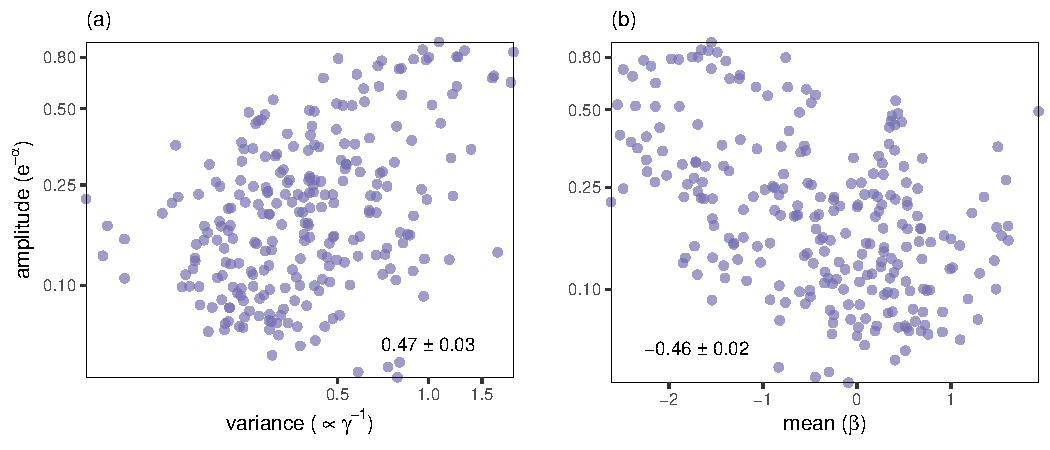
\includegraphics[width=0.9\textwidth]{figures/alpha-vs-gamma-beta}
    	  \vspace{0.3cm}
	   \caption{Relationship between the posterior distributions for parameters $\alpha_i$, $\gamma_i$ and $\beta_i$ across species. Panel (a) describes the relationship between the amplitude ($e^{\alpha_i}$) and variance ($\propto\gamma_i^{-1}$) of distributions. Panel (b) describes the relationship between the amplitude ($e^{\alpha_i}$) and mean ($\beta_i$) of distributions. Each point represents the average value of the corresponding posterior distributions for any given species. The value in the bottom-left corner of the plot displays the Pearson's correlation coefficient between the parameters calculated across all samples.}
      \label{sfig:alpha-vs-gammabeta}
\end{figure}

\clearpage

\begin{figure}[ht]
  \centering
    \vspace{0.5cm}
    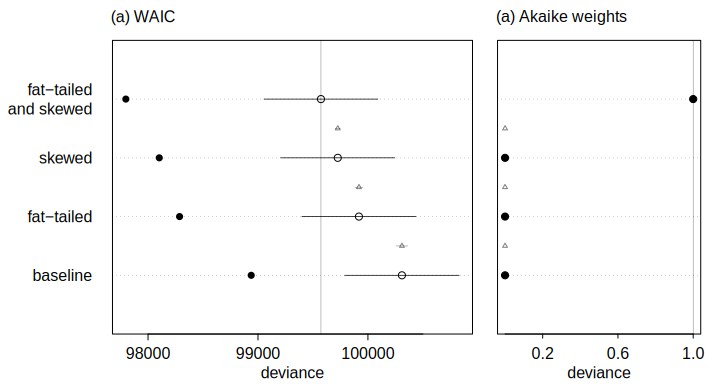
\includegraphics[width=0.85\textwidth]{figures/WAIC-plot}
    	  \vspace{0.3cm}
	   \caption{Comparison of the different models using WAIC values. Each row describes one of the models described in the main text. (a) WAIC comparison of the different models. The filled points are the in-sample deviance of each model, and the open points are the estimated WAIC values. The dark line segments represent the standard error of each WAIC. The standard error of the difference between each WAIC and the best performing model (top row) is characterized by the gray triangles and line segments. The vertical line references the model with the lowest WAIC value. (b) Akaike weight for each model used to compare predictive accuracy of the different Bayesian models (see \citealt{mcelreathStatisticalRethinkingBayesian2020}). According to this measure, the model with fat-tails and skewed response is the best model. The open points are the mean Akaike weights and the line segments represent the corresponding standard error. The vertical line references the model with the highest Akaike weight. These graphs were generated using some of the functions from the R package \textit{rethinking} \citep{mcelreathStatisticalRethinkingBayesian2020}.}
      \label{sfig:WAIC}
\end{figure}

\clearpage

\begin{figure}[ht]
  \centering
    \vspace{0.5cm}
    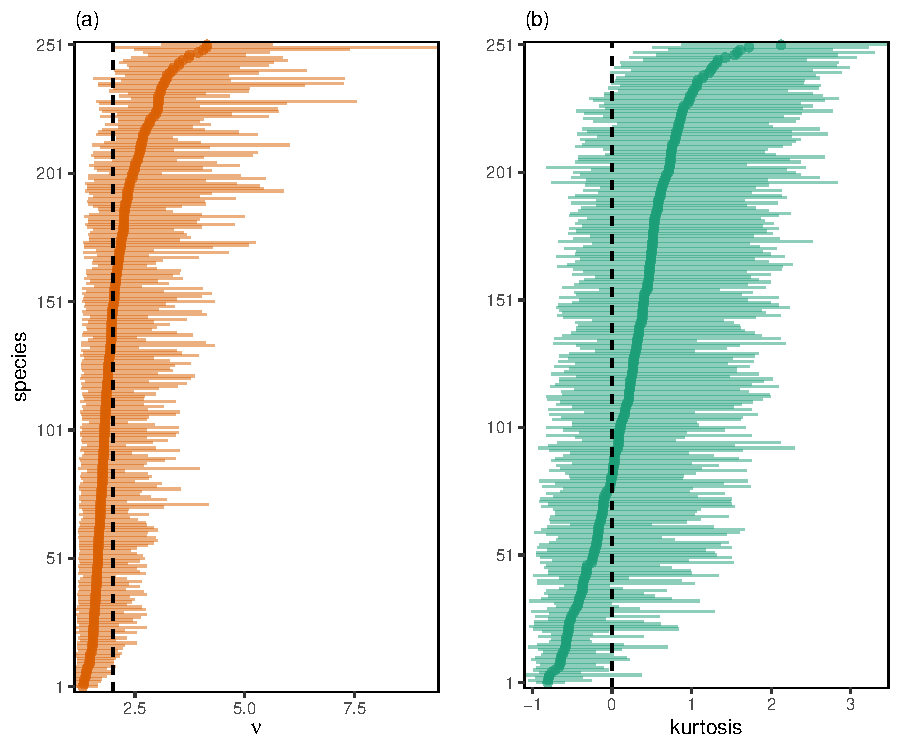
\includegraphics[width=0.85\textwidth]{figures/nu-kurtosis}
    	  \vspace{0.3cm}
	   \caption{Study of the estimates for $\nu_i$ and kurtosis of the distributions. Panel (a) displays the posterior distributions for $\nu_i$ of the 251 species studied. Panel (b) represents the posterior distributions for the kurtosis of the distributions. In both panels, the points represent the mean of the posterior distributions, and the corresponding lines characterize the 89\% confidence intervals. The black dotted lines indicates the $\nu_i$ and kurtosis values corresponding to a normal distribution.}
      \label{sfig:nu-kurtosis}
\end{figure}

\clearpage

\begin{figure}[ht]
  \centering
    \vspace{0.5cm}
    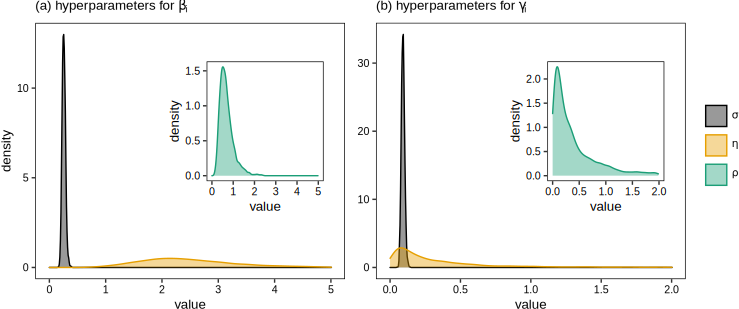
\includegraphics[width=1\textwidth]{figures/hyperparameters-supplementary}
    	  \vspace{0.3cm}
	   \caption{Posterior distributions for the hyperparameters $\eta$, $\rho$ and $\sigma$ characterizing the Gaussian processes in Equations (2) and (3) of the main text. Panels (a) and (b) display the results for $\beta_i$ and $\gamma_i$, respectively.}
      \label{sfig:hyperparameters1}
\end{figure}

\clearpage

\begin{figure}[ht]
  \centering
    \vspace{0.5cm}
    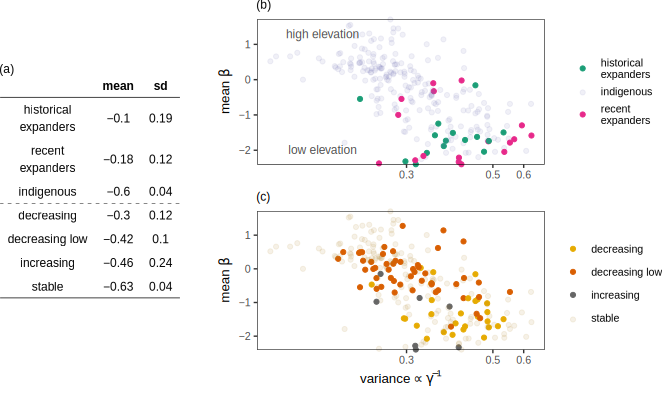
\includegraphics[width=1\textwidth]{figures/Rapaport-species-differences}
    	  \vspace{0.3cm}
	   \caption{Universality of the relationship between mean and variance of species' distributions. Comparison between how different types of species are mapped in Fig.~2a of the main text. Panel (a) describes the correlation coefficient between $\beta_i$ and $\gamma_i$ for each type of species. Panel (b) shows the differences in the way indigenous species, historical expanders and recent expanders are distributed along the environmental gradient. Panel (c) shows the same differences for species with populations that have decreased, decreased in low elevations, increase and remain stable over the last decades (see Supplementary Table 1 for further details).}
      \label{sfig:rapaport-types}
\end{figure}

\clearpage

\begin{figure}[ht]
  \centering
    \vspace{0.5cm}
    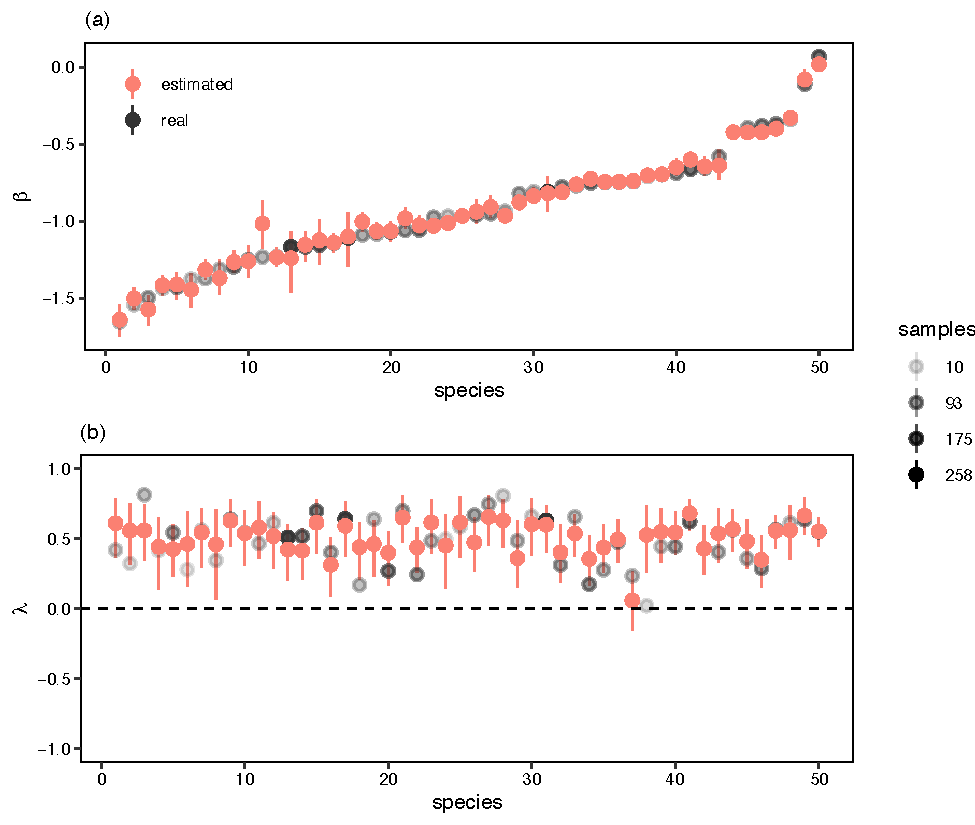
\includegraphics[width=0.85\textwidth]{figures/lambda-test}
    	  \vspace{0.3cm}
	   \caption{Testing the model's ability to estimate $\lambda_i$ with simulated data. We generated 50 fat-tailed and skewed distributions along an environmental axis, randomly sampling the different parameter values $\alpha_i$, $\beta_i$, $\gamma_i$, $\nu_i$, and $\lambda_i$ (see Code Availability section for further information). Then we used these distributions to simulate presence/absence data along the environmental axis using a binomial distribution, and used the model described in Eq.~(6) of the main text to estimate the posterior distributions for the different parameters. The different panels showcase the comparison between real parameter values (black) and the posterior distributions (red) for (a) $\beta_i$ and (b) $\lambda_i$. The transparency for the points describing the real parameter values provides an indication of the sample size of each simulated species (number of occurrences). The red dots and red bars characterize the mean and the $89\%$ confidence intervals for the different posterior distributions, respectively. The black-dotted line indicates the $\lambda_i$ value characterizing a normal distribution.}
      \label{sfig:simulated-lambdas}
\end{figure}

\clearpage

\begin{figure}[ht]
  \centering
    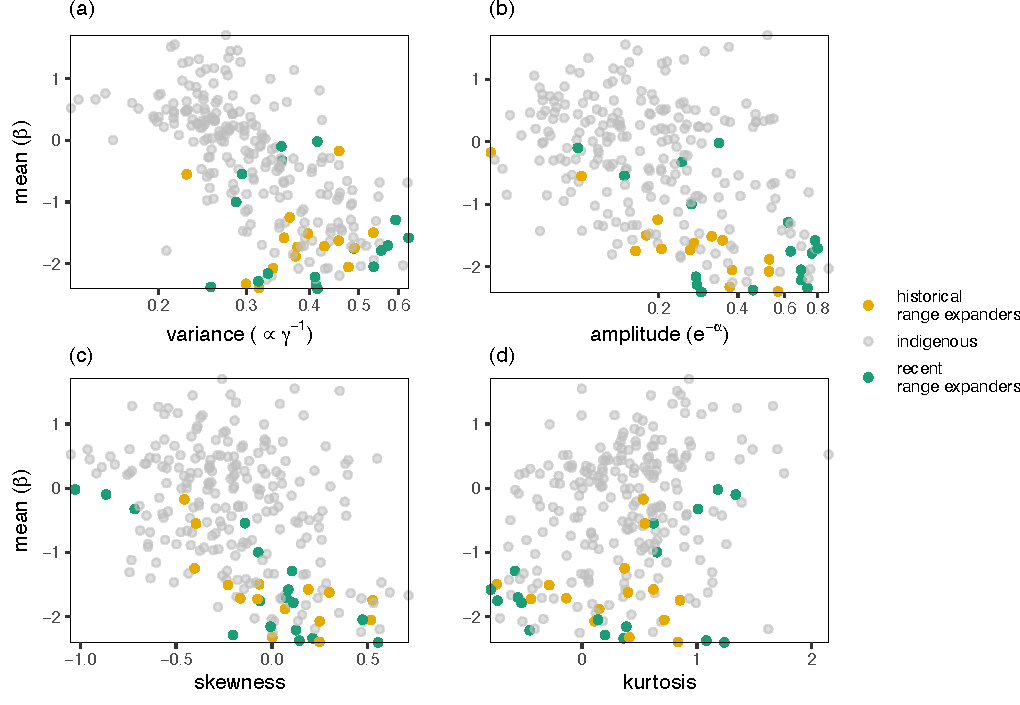
\includegraphics[width=0.9\textwidth]{figures/categorical-figure3}
    	  \vspace{0.1cm}
	   \caption{Comparing the distributions of different types of species. These results are analogous results to those displayed in Fig.~4 of the main text, but they were obtained using ordinal measures of abundance instead of presence/absence data. Focussing on the differences between indigenous, historical range expanding and recent range expanding species, the panels describe the relationship between the basic properties of their distributions. Panels (a-d) characterize the relationship between the mean, and the variance, amplitude, skewness and kurtosis of the species' distributions (Supplementary Table 2 and \citealt{kermanSkewnessKurtosisBounds2013}). The points in every panel are calculated as the average value across all samples of the model. %The analogous results found for species classified accroding to their population change tendency over the years is presented in Supplementary Fig~XX. The ellipses characterize the 1 standard deviation ellipses for each species type. 
	   }
	   %7-4.5
      \label{sfig:figure3-categorical}
\end{figure}

\clearpage

\begin{figure}[ht]
  \centering
    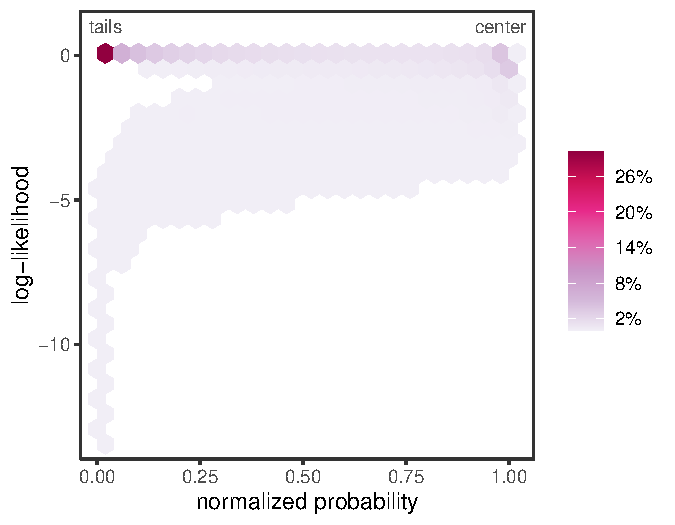
\includegraphics[width=0.5\textwidth]{figures/loglik-all-bin}
    	  \vspace{0.1cm}
	   \caption{Studying the distribution of log-likelihood values. The graph maps the log-likelihood and normalized probability values for all species across all samples. The colour characterizes the overall percentage of points falling within a given hexagon.}
	   %5-4
      \label{sfig:loglik-all}
\end{figure}

\clearpage

\begin{figure}[ht]
  \centering
    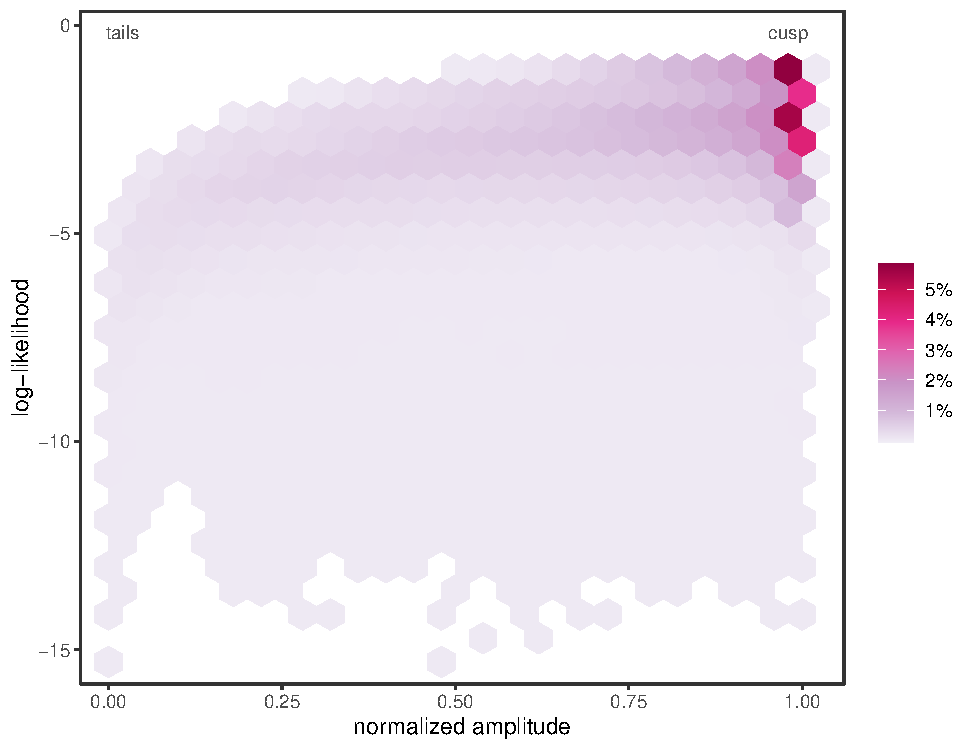
\includegraphics[width=0.5\textwidth]{figures/loglik-notshow}
    	  \vspace{0.1cm}
	   \caption{Studying the distribution of log-likelihood values. These results are analogous results to those displayed in Fig.~5 of the main text, but they were obtained using ordinal measures of abundance instead of presence/absence data. The graph maps the log-likelihood and normalized probability values for all species across all samples. The colour characterizes the overall percentage of points falling within a given hexagon. Notice that in this figure there are only displayed those points that present a likelihood smaller than $0.5$.}
	   %5-4
      \label{sfig:loglik-all-categorical}
\end{figure}

\clearpage

\section*{Supplementary Tables}

\begin{table}[ht]
\begin{center}
\begin{tabular}{ p{8em} p{6em} l p{16em}} 
\textbf{Information} & \textbf{Variable type} & \textbf{Variable} & \textbf{Description} \\
\hline
\multirow{3}{7em}{ecological indicator values} & \multirow{3}{6em}{climate indicators} & temperature & \textit{10 classes ranging from alpine climates to very warm collines} \\
& & continentality & \textit{5 classes ranging from oceanic to continental climates}\\ 
& & light & \textit{5 classes ranging from deep shade to full light}\\ 
\cline{2-4}
& \multirow{5}{6em}{soil indicators} & moisture & \textit{10 classes ranging from very dry to flooded soil} \\
& & reaction & \textit{5 classes ranging from extremely acid to alkaline soil} \\
& & nutrients & \textit{5 classes ranging from very infertile to over-rich soils} \\ 
& & humus & \textit{5 classes ranging from little to high humus content} \\
& & aeration & \textit{5 classes ranging from bad to good aeration} \\ 
\hline
\multirow{3}{7em}{range of variation} & \multirow{3}{6em}{climate indicators} & temperature & \multirow{3}{14em}{\textit{3 classes indicating small, large and unlimited variation of the different climatic indicators}} \\  
& & continentality & \\ 
& & light & \\ 
\cline{2-4}
& \multirow{3}{6em}{soil indicators} & moisture & \multirow{5}{14em}{\textit{3 classes indicating small, large and unlimited variation of the different soil indicators}}  \\ 
& & reaction & \\ 
& & nutrients & \\ 
& & humus & \\ 
& & aeration & \\ 
\hline
\multirow{3}{7em}{species types} & \multirow{2}{6em}{time of immigration} & invasion status & \textit{classified as indigenous, historical range expanders and recent range expanders} \\  
& \makecell[l]{ \\change\\tendency} & abundance & \textit{classified as stable, decreasing, decreasing at low elevations, and increasing in abundance}\\ 
\hline  
\end{tabular}
\end{center}
\caption{Description of the different plant attributes obtained form \citealt{landoltFloraIndicativaOkologische2010}. Each row describe one of the variables used, including the variable type, name in the database, and number of classes for such variable.}
\label{stab:EI}   
\end{table}

\clearpage


\begin{table}[ht]
\begin{center}
\begin{tabular}{  p{6em} | p{1em} l l } 
\textbf{response curve} & &  \(\beta^{\prime}_i\) & \(\gamma^{\prime}_i\) \\
\\[-1em]
\hline
\\[-1em]
baseline & & \(\beta_i\) & \(\gamma_i\) \\
\\[-1em]

\\[-1em]
fat-tailed & & \(\beta_i\) & \( g = \sqrt{\frac{\gamma_i \Gamma\left(\frac{3}{\nu_i}\right)}{\Gamma\left(\frac{1}{\nu_i}\right)}}\) \\
\\[-1em]

\\[-1em]
skewed &  & \( q_2 = \beta_i - \frac{2 \lambda_i}{\sqrt{\pi} \gamma^{\prime}_i}  \)  & \( q_1 = \gamma_i  \sqrt{\frac{\pi\left(1+3 \lambda^{2}_{i}\right)-8\lambda^2_i}{2\pi}}  \)  \\
\\[-1em]
  
\\[-1em]
\multirow{-1.25}{6em}{skewed and fat-tailed} & & \( f_2 = \beta_i - \frac{2^{\frac{2}{\nu_i}}\lambda_i \Gamma\left(\frac{1}{2}+\frac{1}{\nu_i}\right)}{\sqrt{\pi}\gamma^{\prime}_i}   \)  & \( f_1 = \gamma_i \sqrt{\frac{\pi \left(1+3\lambda^2_i\right) \Gamma\left(\frac{3}{\nu_i}\right)-16^{\frac{1}{\nu_i}} \lambda^{2}_{i} \Gamma\left(\frac{1}{2}+\frac{1}{\nu_i}\right)^2 \Gamma\left(\frac{1}{\nu_i}\right)}{\pi \Gamma\left(\frac{1}{\nu_i}\right)}} \) \\
\\[-1em]
  
\end{tabular}
\end{center}
Additional definitions for the different models used. Except for the baseline model, all models are described in terms of $\beta^{\prime}_i$ and $\gamma^{\prime}_i$. However these models are parametrized using instead $\alpha_i$, $\beta_i$, $\gamma_i$, $\nu_i$ and $\lambda_i$, which are parameters that are comparable across models. The relationship between all parameters is described in the table (see \citealt{kermanSkewnessKurtosisBounds2013} for further details, including the analytical expressions for the kurtosis and skewness of all distributions).
\label{stab:formulas}   
\end{table}

\clearpage


\bibliography{references2}

\end{document}
